\documentclass[aspectratio=169,11pt]{beamer}
% Compiles with pdflatex (+ bibtex) and with Tectonic/XeLaTeX. Sources are ASCII-only.
\usepackage{iftex}
\ifPDFTeX
  \usepackage[utf8]{inputenc}
  \usepackage[T1]{fontenc}
\fi
% shared packages, notation and generated numbers for the end-evaluation report, slides and appendix
\usepackage{amsmath,amssymb}
\usepackage{booktabs}
\usepackage{graphicx}
\usepackage{siunitx}
\usepackage{xcolor}
\usepackage{adjustbox}
\makeatletter
\providecommand{\input@path}{}
\g@addto@macro\input@path{{.}{docs/}{./docs/}{../docs/}}
\makeatother
\graphicspath{{../figures/nine_crop/}{../figures/four_crop/}{figures/nine_crop/}}
% generated by code/19_endeval_tex.py -- do not edit
\newcommand{\nPairs}{59}
\newcommand{\nCountries}{20}
\newcommand{\nCrops}{9}
\newcommand{\orderEq}{Wheat $>$ Maize $>$ Common bean $>$ Soybean $>$ Rapeseed-mustard $>$ Chickpea $>$ Rice $>$ Lentil $>$ Groundnut}
\newcommand{\topEq}{Wheat}
\newcommand{\secondEq}{Maize}
\newcommand{\lastEq}{Groundnut}
\newcommand{\topEqValue}{0.0563}
\newcommand{\secondEqValue}{0.0297}
\newcommand{\orderPw}{Wheat $>$ Common bean $>$ Chickpea $>$ Rapeseed-mustard $>$ Soybean $>$ Maize $>$ Lentil $>$ Groundnut $>$ Rice}
\newcommand{\topPw}{Wheat}
\newcommand{\secondPw}{Common bean}
\newcommand{\lastPw}{Rice}
\newcommand{\topPwValue}{0.0696}
\newcommand{\secondPwValue}{0.0233}
\newcommand{\topPairA}{wheat--Russia}
\newcommand{\topPairAValue}{0.1315}
\newcommand{\topPairB}{maize--South Africa}
\newcommand{\topPairBValue}{0.1237}
\newcommand{\topPairC}{wheat--USA}
\newcommand{\topPairCValue}{0.0903}
\newcommand{\topPairD}{wheat--India}
\newcommand{\topPairDValue}{0.0676}
\newcommand{\topPairE}{common bean--Brazil}
\newcommand{\topPairEValue}{0.0459}
\newcommand{\topPairF}{common bean--Tanzania}
\newcommand{\topPairFValue}{0.0357}
\newcommand{\refHeatPair}{common bean--India}
\newcommand{\refHeat}{5.046}
\newcommand{\refWaterPair}{chickpea--India}
\newcommand{\refWater}{0.789}
\newcommand{\refImpPair}{rice--Bangladesh}
\newcommand{\refImp}{0.421}
\newcommand{\groupOrder}{Cereals $>$ Pulses $>$ Oilseeds}
\newcommand{\nDivUnits}{21}
\newcommand{\wheatTopZinc}{16}
\newcommand{\wheatTopIron}{15}
\newcommand{\wheatTopProtein}{9}
\newcommand{\wheatTopKcal}{14}
\newcommand{\maizeSAkcal}{22}
\newcommand{\maizeSArainfed}{89}
\newcommand{\maizeSAEwater}{0.46}
\newcommand{\maizeUAEwater}{0.61}
\newcommand{\maizeFoodUSA}{1}
\newcommand{\maizeFoodChina}{3}
\newcommand{\maizeFoodSA}{40}
\newcommand{\futHeatShare}{72}
\newcommand{\futWaterShare}{28}
\newcommand{\nPairsDown}{14}
\newcommand{\nPairsDownWaterOnly}{14}
\newcommand{\futOrderEq}{Wheat $>$ Maize $>$ Common bean $>$ Rapeseed-mustard $>$ Soybean $>$ Chickpea $>$ Rice $>$ Lentil $>$ Groundnut}
\newcommand{\histOrderEq}{Wheat $>$ Maize $>$ Common bean $>$ Soybean $>$ Rapeseed-mustard $>$ Chickpea $>$ Rice $>$ Groundnut $>$ Lentil}
\newcommand{\futOrderPw}{Wheat $>$ Common bean $>$ Chickpea $>$ Rapeseed-mustard $>$ Soybean $>$ Maize $>$ Lentil $>$ Groundnut $>$ Rice}
\newcommand{\nPairsUp}{40}
\newcommand{\nPairsExceedRef}{1}
\newcommand{\meanDTeff}{1.9}
\newcommand{\futTopPair}{wheat--Russia}
\newcommand{\futTopPairChange}{+0.0207}
\newcommand{\climCheckSameSign}{92}
\newcommand{\climCheckRho}{0.96}
\newcommand{\histReproMaxDiff}{4.3e-06}
\newcommand{\shockTopMar}{maize--South Africa}
\newcommand{\shockTopMarValue}{-0.53}
\newcommand{\shockTopKcal}{rice--Bangladesh}
\newcommand{\shockTopKcalValue}{-6.3}
\newcommand{\shockZeroMar}{40}
\newcommand{\shockN}{59}
\newcommand{\passOldN}{43}
\newcommand{\passOldPos}{17}
\newcommand{\passNewN}{49}
\newcommand{\passNewPos}{5}
\newcommand{\nIronShort}{7}
\newcommand{\nIronShortAlt}{0}
\newcommand{\nZincShort}{0}
\newcommand{\nZincShortAlt}{0}
\newcommand{\nAdqCountries}{20}
\newcommand{\futYieldWorst}{Common bean}
\newcommand{\futYieldWorstValue}{-17.8}
\newcommand{\futNutTopPair}{common bean--Brazil}
\newcommand{\futNutTopMar}{-0.66}
\newcommand{\corrLitEmp}{-0.04}
\newcommand{\robN}{184}
\newcommand{\robTopAll}{178}
\newcommand{\robTopFfour}{44}
\newcommand{\robNFfour}{46}
\newcommand{\mcTop}{Wheat}
\newcommand{\mcTopShare}{92.0}
\newcommand{\mcSecond}{Maize}
\newcommand{\mcSecondShare}{6.0}
\newcommand{\zhaoRhoFfour}{+0.6}
\newcommand{\zhaoRhoClimate}{+0.8}
\newcommand{\shockRho}{+0.35}
\newcommand{\shockP}{0.00}
\newcommand{\shockNpairs}{59}
\newcommand{\oosMedian}{0.33}
\newcommand{\oosPos}{28}
\newcommand{\oosN}{35}
\newcommand{\presentHeatShare}{9}
\newcommand{\presentWaterShare}{91}
\newcommand{\nTopSevenWater}{7}
\newcommand{\empHeatDetected}{22}
\newcommand{\empHeatCountry}{8}
\newcommand{\empN}{59}
\newcommand{\litN}{12}
\newcommand{\litAgree}{7}
\newcommand{\litDiffer}{2}
\newcommand{\litPartial}{1}
\newcommand{\litOther}{2}
\newcommand{\orderMidEq}{Wheat $>$ Maize $>$ Soybean $>$ Rice}
\newcommand{\orderOrigMidEq}{Wheat $>$ Maize $>$ Soybean $>$ Rice}
\newcommand{\orderMidPw}{Wheat $>$ Soybean $>$ Maize $>$ Rice}
\newcommand{\orderOrigMidPw}{Wheat $>$ Soybean $>$ Maize $>$ Rice}
\newcommand{\orderFourEq}{Wheat $>$ Maize $>$ Soybean $>$ Rice}
\newcommand{\orderOrigFourEq}{Wheat $>$ Maize $>$ Soybean $>$ Rice}
\newcommand{\orderFourPw}{Wheat $>$ Soybean $>$ Maize $>$ Rice}
\newcommand{\orderOrigFourPw}{Wheat $>$ Soybean $>$ Maize $>$ Rice}
\newcommand{\orderNineEq}{Wheat $>$ Maize $>$ Bean $>$ Soybean $>$ Rapeseed $>$ Chickpea $>$ Rice $>$ Lentil $>$ Groundnut}
\newcommand{\orderOrigNineEq}{Wheat $>$ Maize $>$ Soybean $>$ Rice}
\newcommand{\orderNinePw}{Wheat $>$ Bean $>$ Chickpea $>$ Rapeseed $>$ Soybean $>$ Maize $>$ Lentil $>$ Groundnut $>$ Rice}
\newcommand{\orderOrigNinePw}{Wheat $>$ Soybean $>$ Maize $>$ Rice}
\newcommand{\litTopPair}{wheat--Russia}
\newcommand{\litTopValue}{0.2099}
\newcommand{\litSecondPair}{wheat--India}
\newcommand{\litSecondValue}{0.2076}
\newcommand{\litRatioMedian}{1.76}
\newcommand{\exFourLheatc}{0.580}
\newcommand{\exFourmaxLheat}{0.580}
\newcommand{\exFourEheat}{1.000}
\newcommand{\exFourLwater}{0.178}
\newcommand{\exFourmaxLwater}{0.546}
\newcommand{\exFourEwater}{0.327}
\newcommand{\exFoursTpc}{0.100}
\newcommand{\exFourmaxsT}{0.200}
\newcommand{\exFourSheat}{0.500}
\newcommand{\exFourKy}{1.10}
\newcommand{\exFourmaxKy}{1.25}
\newcommand{\exFourSwater}{0.880}
\newcommand{\exFourI}{0.222}
\newcommand{\exFourmaxI}{0.421}
\newcommand{\exFourInorm}{0.527}
\newcommand{\exFourFFourpipeline}{0.2076}
\newcommand{\exNineLheatc}{0.580}
\newcommand{\exNinemaxLheat}{5.046}
\newcommand{\exNineEheat}{0.115}
\newcommand{\exNineLwater}{0.178}
\newcommand{\exNinemaxLwater}{0.789}
\newcommand{\exNineEwater}{0.226}
\newcommand{\exNinesTpc}{0.100}
\newcommand{\exNinemaxsT}{0.200}
\newcommand{\exNineSheat}{0.500}
\newcommand{\exNineKy}{1.10}
\newcommand{\exNinemaxKy}{1.25}
\newcommand{\exNineSwater}{0.880}
\newcommand{\exNineI}{0.222}
\newcommand{\exNinemaxI}{0.421}
\newcommand{\exNineInorm}{0.527}
\newcommand{\exNineFFourpipeline}{0.0676}

\InputIfFileExists{nine_crop/generated/numbers_india.tex}{}{}

\definecolor{ink}{HTML}{222222}
\definecolor{muted}{HTML}{6B6B6B}
\definecolor{paddy}{HTML}{1F4E3D}
\definecolor{grain}{HTML}{C8961A}
\definecolor{clay}{HTML}{B5523B}
\definecolor{cereal}{HTML}{2A78D6}
\definecolor{pulse}{HTML}{EB6834}
\definecolor{oilseed}{HTML}{1BAF7A}
\newcommand{\Teff}{\ensuremath{T_{\mathrm{eff}}}}
\newcommand{\Tcrit}{\ensuremath{T_{\mathrm{crit}}}}
\newcommand{\ETc}{\ensuremath{\mathrm{ET_c}}}
\newcommand{\ETo}{\ensuremath{\mathrm{ET_0}}}
\newcommand{\Fd}{\ensuremath{\mathrm{F4}}}

\usepackage[round]{natbib}
\bibliographystyle{plainnat}
\hypersetup{colorlinks=true,linkcolor=paddy,citecolor=paddy,urlcolor=paddy}
\usetheme{default}
\setbeamercolor{structure}{fg=paddy}
\setbeamercolor{frametitle}{fg=paddy}
\setbeamercolor{title}{fg=paddy}
\setbeamercolor{alerted text}{fg=clay}
\setbeamercolor{block title}{bg=paddy,fg=white}
\setbeamercolor{block body}{bg=paddy!6}
\setbeamercolor{block title alerted}{bg=clay,fg=white}
\setbeamercolor{block body alerted}{bg=clay!7}
\setbeamerfont{frametitle}{series=\bfseries,size=\large}
\setbeamertemplate{navigation symbols}{}
\setbeamertemplate{itemize items}[circle]
\setbeamertemplate{footline}{\hfill{\scriptsize\color{muted}\insertframenumber\,/\,\inserttotalframenumber}\hspace*{1em}\vspace*{0.6em}}
\setbeamertemplate{frametitle}{\vspace*{0.4em}\insertframetitle\par\vspace*{-0.2em}{\color{grain}\rule{2.2em}{2pt}}}
\newcommand{\src}[1]{\par\vfill{\tiny\color{muted}#1}}

\title{Climate Change and Nutritional Security:\\ Which Crops Are Most Vulnerable?}
\subtitle{End evaluation}
\author{Arpit Mahtele \and Dev Patel \and Navey Puri \and Shreyash Lohare}
\date{Earth 616}

\begin{document}
\begin{frame}\titlepage\end{frame}

\begin{frame}{The question, and what is new since the mid-evaluation}
\begin{columns}[T]
\column{0.5\textwidth}
\textbf{Questions}
\begin{enumerate}
\item Which crop is most vulnerable to climate, given what it supplies to diets?
\item If its yield falls, what happens to nutrient supply?
\end{enumerate}
\textbf{Gap:} yield studies and nutrient studies are separate; no reviewed study combines exposure,
sensitivity and nutritional importance in one index.
\column{0.5\textwidth}
\textbf{Done for the end evaluation}
\begin{itemize}
\item Presented method (literature-only sensitivity) implemented everywhere
\item 4 $\to$ \nCrops\ crops: cereals, pulses, oilseeds; \nPairs\ crop--country pairs
\item Future 2041--2060 with comparable processing
\item Nutrition consequences, robustness, validation, literature comparison
\item India and Hyderabad: what the index means locally
\end{itemize}
\end{columns}
\end{frame}

\begin{frame}{The index: what a high score means}
\[
\Fd = \tfrac12\big(\underbrace{E_{\text{heat}}\,S_T}_{\text{heat}} + \underbrace{E_{\text{water}}\,S_P}_{\text{water}}\big)\times\underbrace{\tilde I}_{\text{diet}}
\]
\begin{itemize}
\item $E$: observed stress \emph{level} 2001--24 on the crop's own area --- \si{\celsius} of flowering-season
$\Teff$ above the crop's threshold; rainfed share $\times$ unmet water need $1-P/\ETc$
\item $S$: literature yield loss per unit of stress --- $s_T = 1/(T_{\lim}-\Tcrit)$, FAO $K_y$
\item $\tilde I$: crop's mean share of national energy, protein, fat, zinc, iron (FAO 2021--23)
\end{itemize}
\begin{block}{Reading}
High \Fd\ = the crop is stressed \emph{where it grows}, loses yield fast under that stress, \emph{and} people
depend on it for nutrients. It is a relative score (0--1 scale), never a yield loss.
\end{block}
\end{frame}

\begin{frame}{Five new crops: every input checked against a source}
\centering\scriptsize
\begin{minipage}{\textwidth}\centering
\adjustbox{max width=\textwidth}{\begin{tabular}{lrrrrrrrl}
\toprule
Crop & $T_{crit}$ & $T_{lim}$ & $s_T$ (/\si{\celsius}) & $S_T$ & $K_y$ & $S_P$ & $\bar K_c$ & heat source \\
\midrule
Wheat & 25.0 & 35.0 & 0.100 & 0.50 & 1.10 & 0.88 & 0.88 & Deryng 2014 \\
Rice & 35.0 & -- & 0.070 & 0.35 & 1.25 & 1.00 & 1.11 & Yoshida 1981; Jagadish 2007 \\
Maize & 32.0 & 45.0 & 0.077 & 0.38 & 1.25 & 1.00 & 0.84 & Deryng 2014 \\
Chickpea & 34.0 & 41.1 & 0.140 & 0.70 & 0.88 & 0.70 & 0.77 & Bhandari 2020 (fit) \\
Lentil & 31.9 & 37.8 & 0.170 & 0.85 & 1.00 & 0.80 & 0.83 & Bhandari 2020 (fit) \\
Common bean & 25.5 & 34.5 & 0.111 & 0.56 & 1.15 & 0.92 & 0.85 & Prasad 2002 (fit) \\
Soybean & 35.0 & 40.0 & 0.200 & 1.00 & 0.85 & 0.68 & 0.89 & Deryng 2014 \\
Groundnut & 31.8 & 42.3 & 0.095 & 0.47 & 0.70 & 0.56 & 0.85 & Prasad 2003 (fit) \\
Rapeseed-mustard & 26.5 & 36.5 & 0.100 & 0.50 & 0.90 & 0.72 & 0.78 & Morrison 2002; slope proxy \\
\bottomrule
\end{tabular}
}
\par\vspace{2pt}{\footnotesize $T_{crit}$, $T_{lim}$ in \si{\celsius} of $T_{eff}$. Rice $K_y$ is a proxy (FAO gives none); lentil $K_y$ and the rapeseed slope are proxies; new-crop heat values are fits to chamber or field data (docs/evidence/literature\_verification\_new\_crops.md).}
\end{minipage}

\par\medskip
\begin{minipage}{0.95\textwidth}\scriptsize
\begin{itemize}
\item Heat: fits to chamber/field seed-yield data \citep{prasad2002bean,prasad2003peanut,bhandari2020,morrison2002}; water: FAO $K_y$, field value for chickpea \citep{tari2022}
\item Calendars: Sacks ``Pulses'' puts Indian chickpea in the monsoon (95\% gap-filled) $\Rightarrow$ cool-season rule: rabi sowing in South Asia, spring sowing where winters freeze
\item Chickpea and lentil food supply from FAOSTAT SUA (hidden inside ``Pulses, Other'' in food balances)
\end{itemize}
\end{minipage}
\end{frame}

\begin{frame}{Result 1: wheat is the most vulnerable crop}
\centering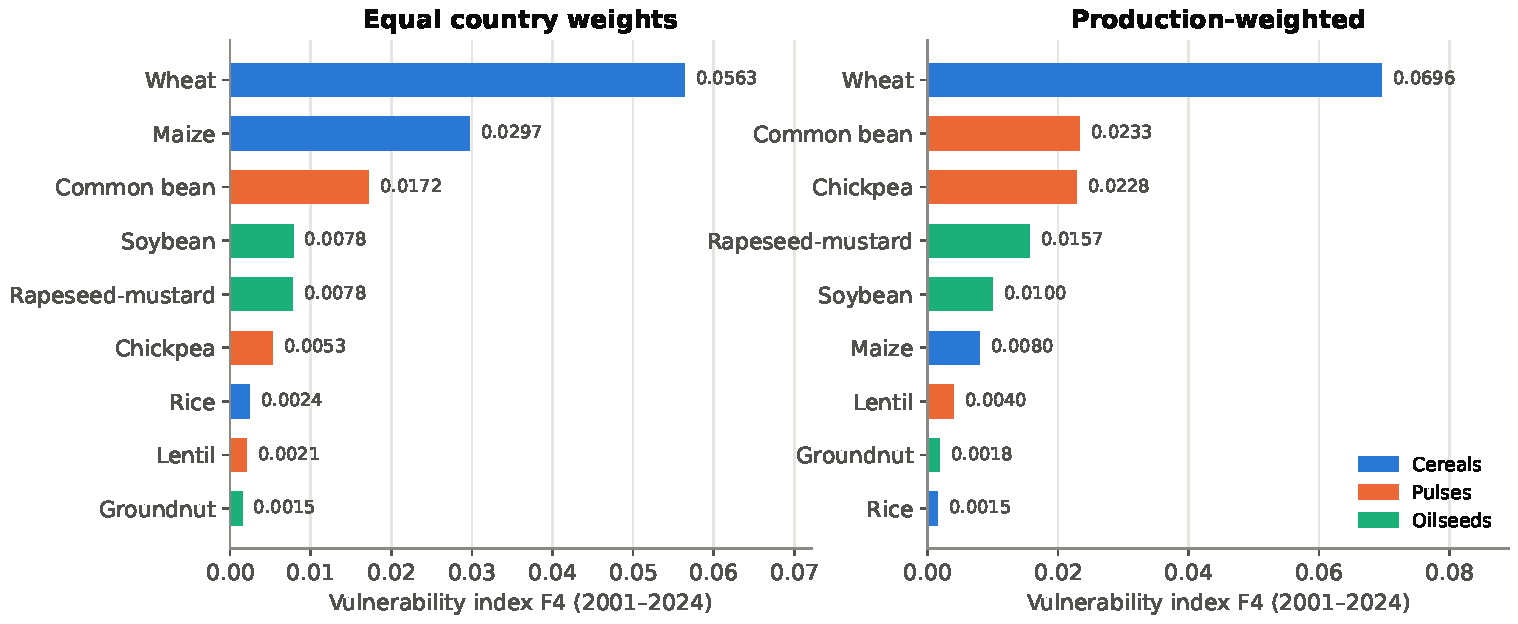
\includegraphics[width=0.93\linewidth]{G01_crop_ranking.pdf}
\src{Equal weights: \orderEq. \quad Production-weighted: \orderPw.}
\end{frame}

\begin{frame}{Where vulnerability sits}
\begin{columns}[T]
\column{0.55\textwidth}
\centering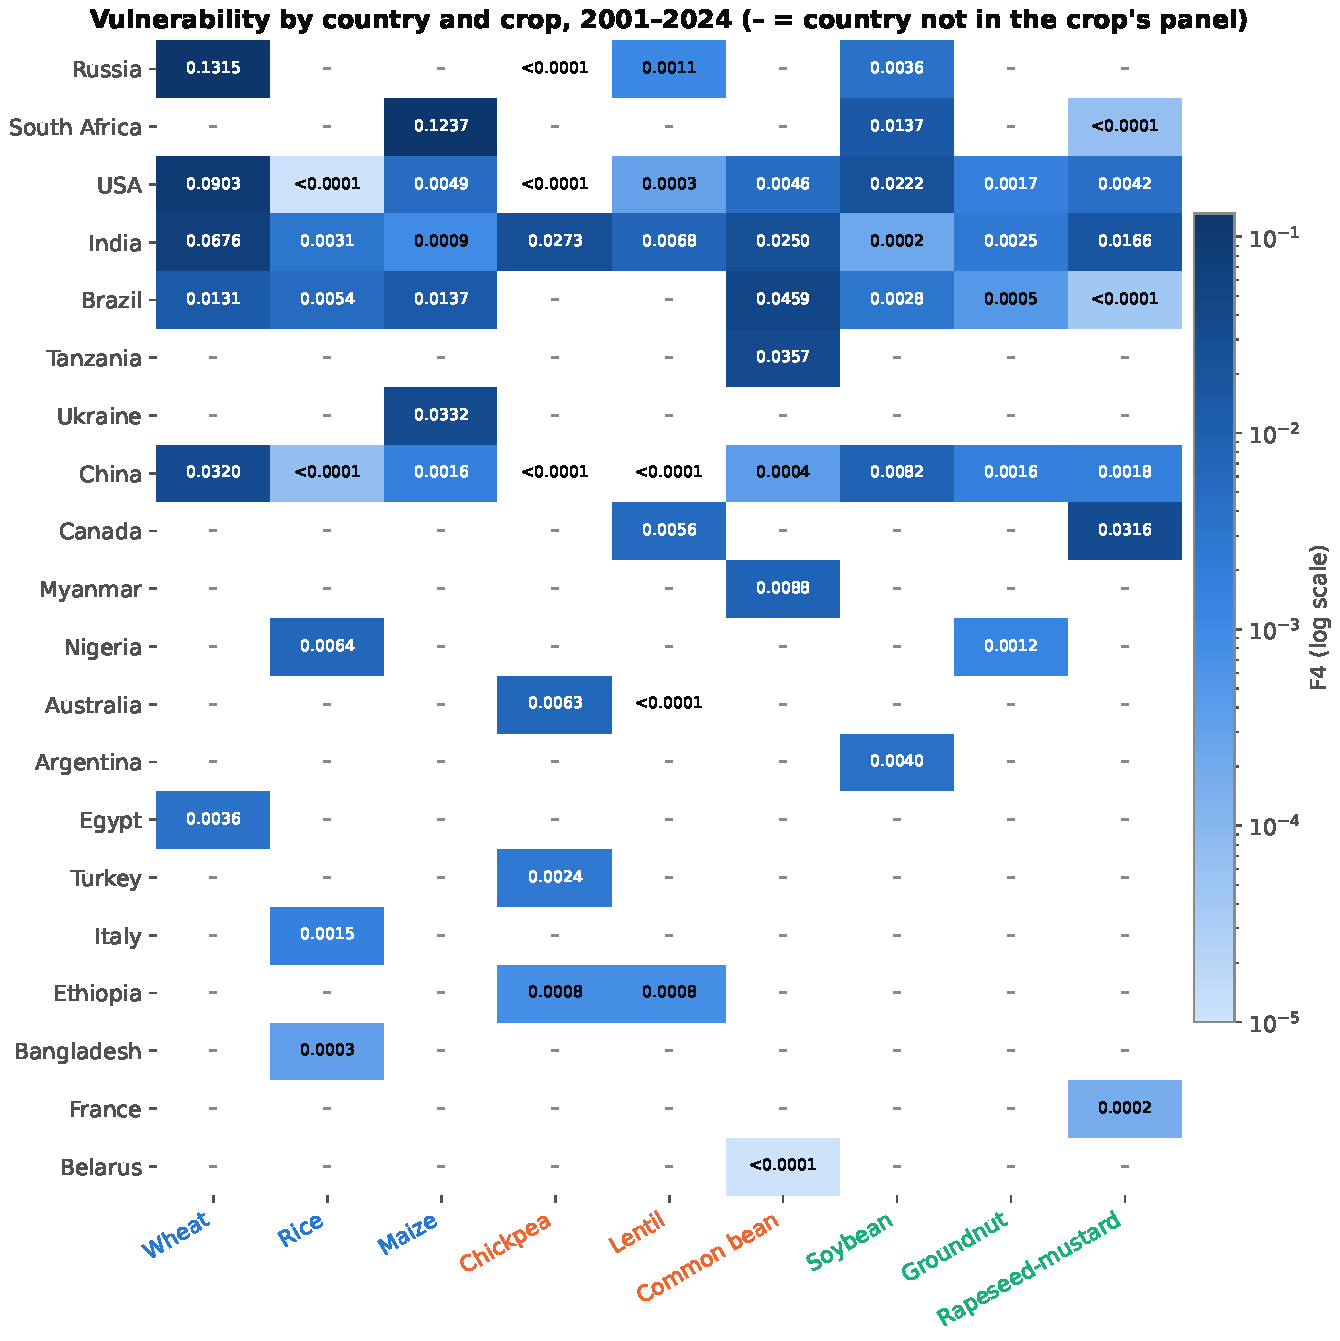
\includegraphics[height=0.82\textheight]{G02_country_crop_matrix.pdf}
\column{0.45\textwidth}\small
Highest pairs:
\begin{itemize}
\item \topPairA\ (\topPairAValue), \topPairC\ (\topPairCValue)
\item \topPairB\ (\topPairBValue): rainfed staple (\maizeSAkcal\% of energy)
\item \topPairD\ (\topPairDValue): also the hottest wheat area
\item \topPairE, \topPairF
\end{itemize}
\textbf{Pattern:} a crop that matters in the diet, grown on rainfed land. Water term larger than heat in
\nTopSevenWater\ of the top 7; today water is \presentWaterShare\% of the summed score, heat drives the future rise.
\end{columns}
\end{frame}

\begin{frame}{Why: overlap, not sensitivity alone}
\centering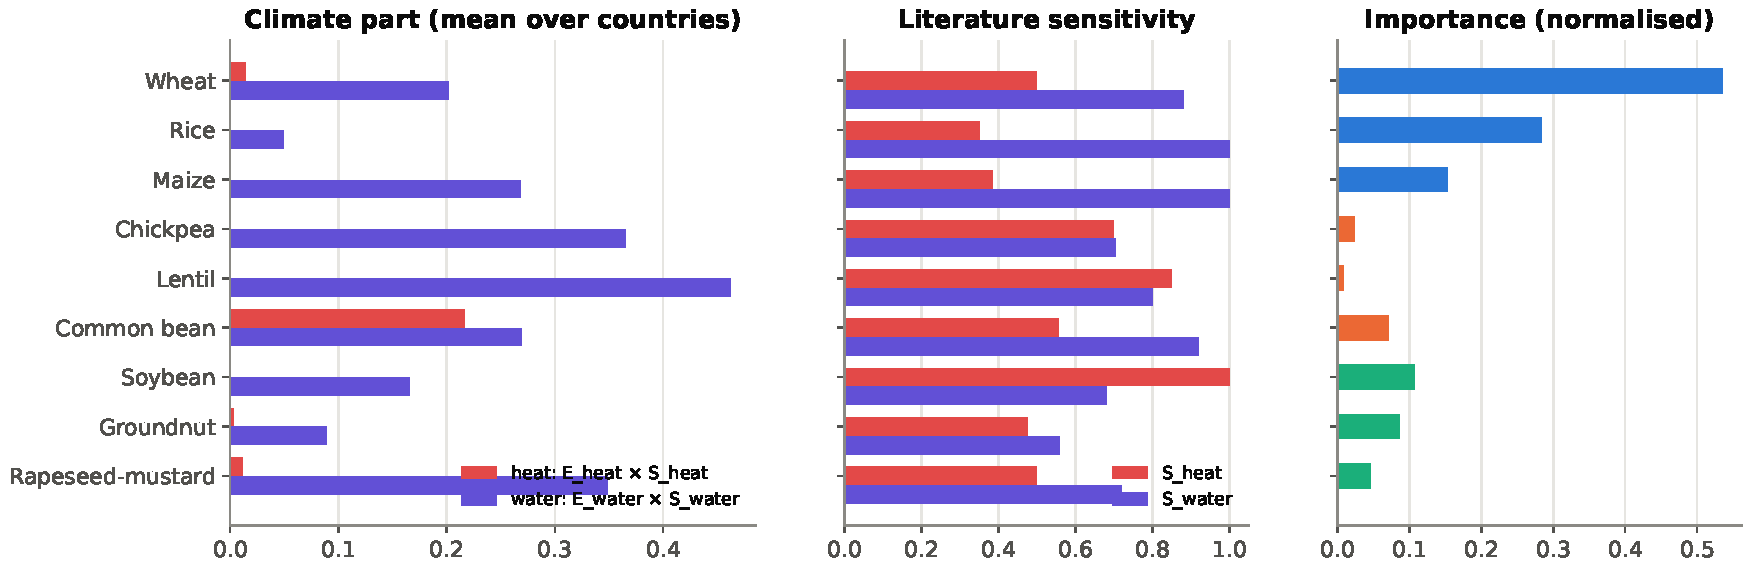
\includegraphics[width=0.95\linewidth]{G03_components.pdf}
\begin{itemize}\small
\item Soybean has the steepest heat slope but zero heat exposure in all its countries; eaten mainly as oil
\item Wheat: largest food source of zinc in \wheatTopZinc\ and iron in \wheatTopIron\ of \nDivUnits\ units; exposed on both hazards
\item Rice scores low because it is irrigated and monthly data hide hot days --- not proven safe
\end{itemize}
\end{frame}

\begin{frame}{Crop groups}
\centering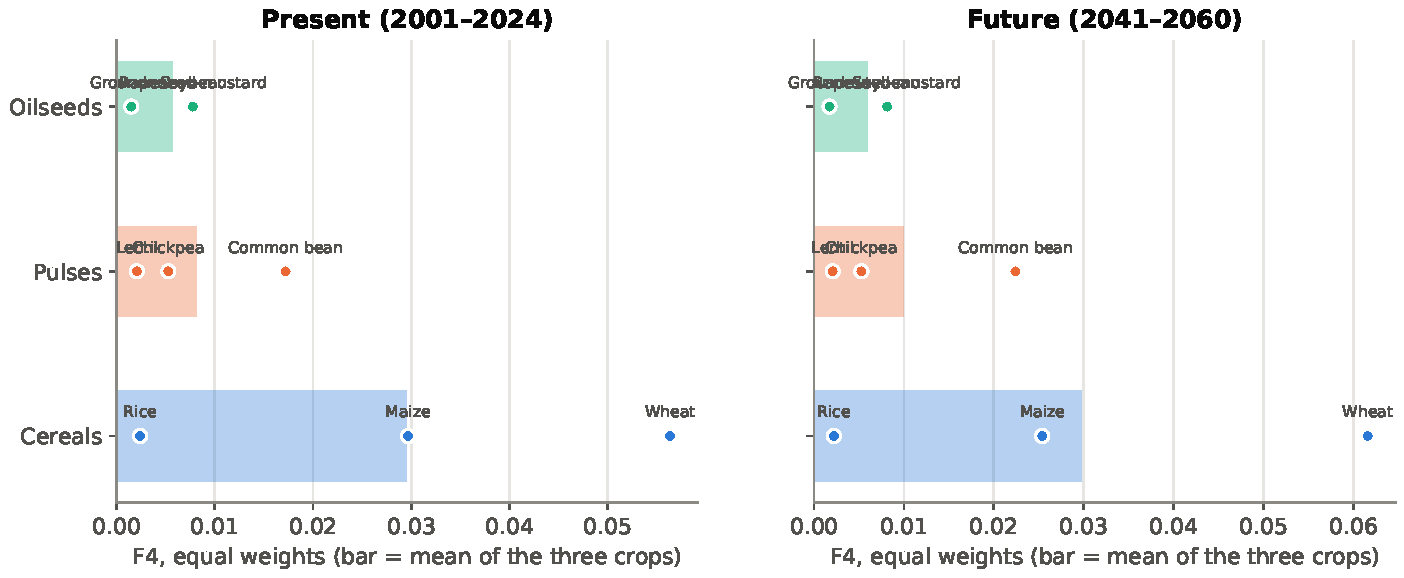
\includegraphics[width=0.9\linewidth]{G06_crop_groups.pdf}
\src{\groupOrder. Group = mean of the three selected crops; it does not describe every cereal, pulse or oilseed.}
\end{frame}

\begin{frame}{Future: comparable processing}
\begin{itemize}
\item WorldClim CMIP6 MRI-ESM2-0, SSP2-4.5, 2041--2060: 20-year monthly climatologies
\item Threshold on an average $\neq$ average of yearly exceedances $\Rightarrow$ change factors added to each
1971--2000 year; historical comparator = same years, same code (reproduces the main series to \histReproMaxDiff)
\item One fixed normalisation reference (2001--24 maxima); sensitivity, importance, crop area held fixed
\item Check: thresholds on the 20-year means give the same sign in \climCheckSameSign\% of pairs ($\rho$ = \climCheckRho)
\end{itemize}
\end{frame}

\begin{frame}{Result 2: by 2041--2060 the order holds, magnitudes rise}
\begin{columns}[T]
\column{0.58\textwidth}
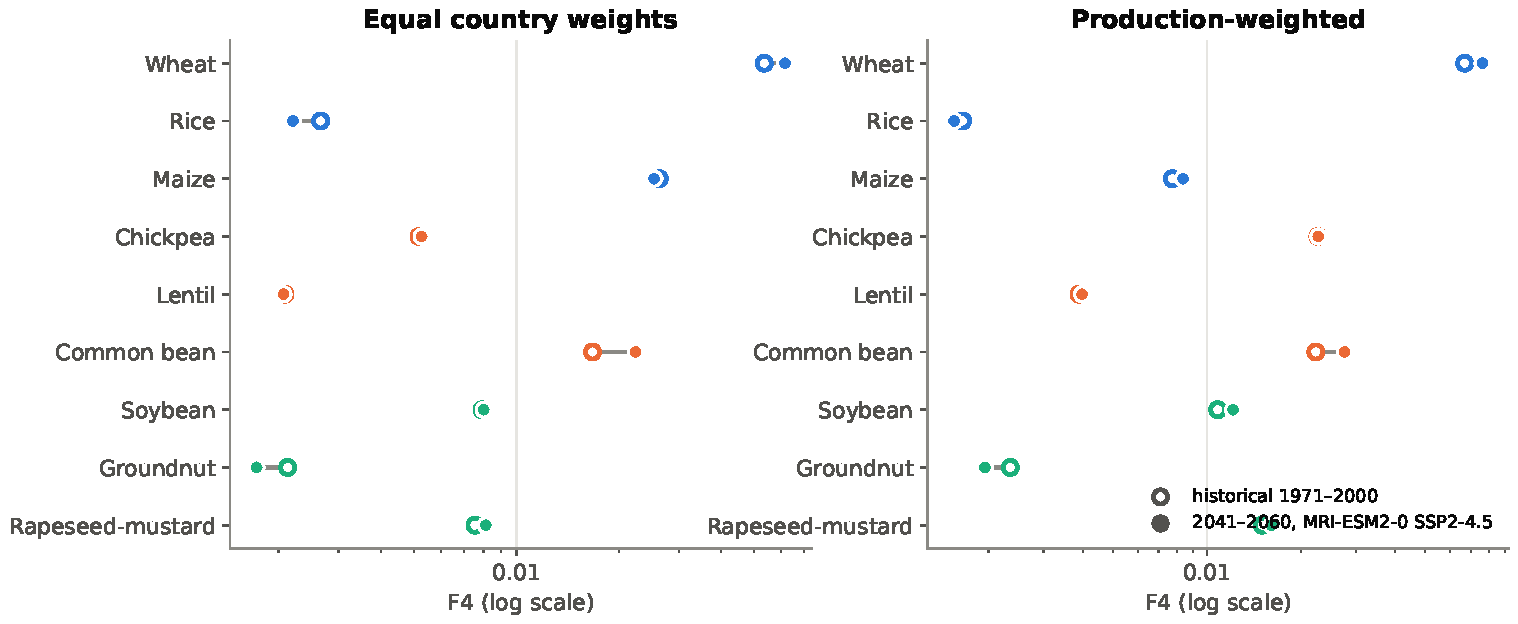
\includegraphics[width=\linewidth]{G04_present_future_crops.pdf}
\column{0.42\textwidth}\small
\begin{itemize}
\item Flowering-season $\Teff$: +\meanDTeff\,\si{\celsius} on average
\item Score rises in \nPairsUp\ of \nPairs\ pairs
\item Increase: \futHeatShare\% heat, \futWaterShare\% water
\item Largest: \futTopPair\ (\futTopPairChange)
\item Falls only where the model gives a smaller rainfed deficit
\end{itemize}
\end{columns}
\src{One model, one scenario: direction under that model, not the range of futures.}
\end{frame}

\begin{frame}{Result 3: the nutrient at stake is iron}
\begin{columns}[T]
\column{0.5\textwidth}
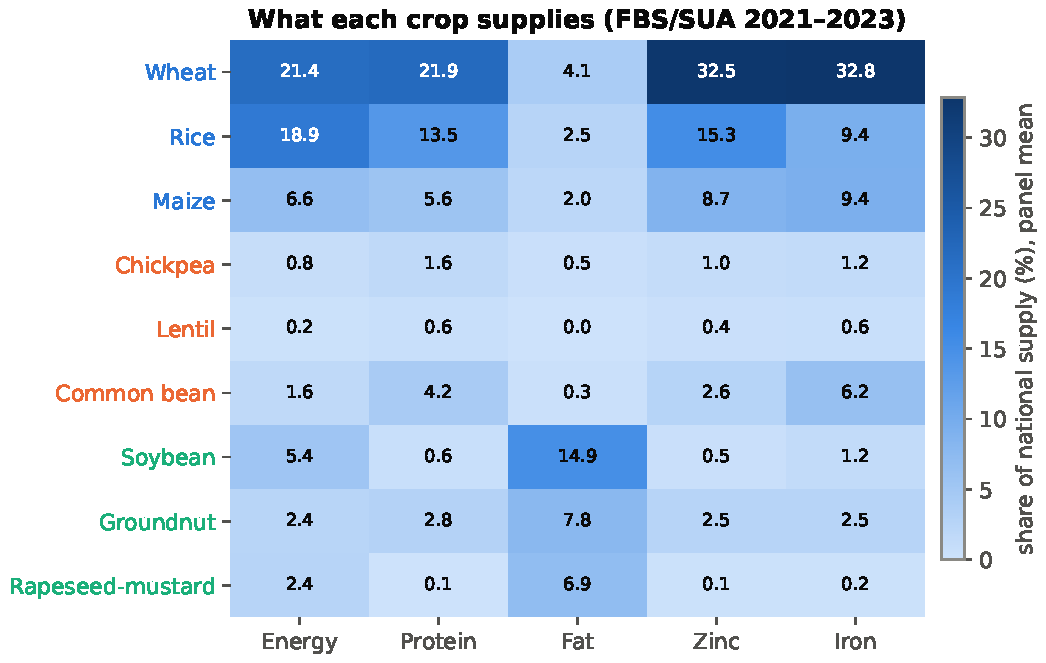
\includegraphics[width=\linewidth]{G07_nutrient_profiles.pdf}
\column{0.5\textwidth}\small
\begin{itemize}
\item Iron is the only nutrient below requirement in any panel country: \nIronShort\ of \nAdqCountries
\item Depends on the requirement: with 15\% bioavailability, \nIronShortAlt\ countries
\item Recommended intakes vs national mean supply: overstates individual shortfall
\item Iron comes mostly from wheat and pulses --- crops among the most vulnerable
\end{itemize}
\end{columns}
\end{frame}

\begin{frame}{A 10\% yield loss: what the diet loses}
\centering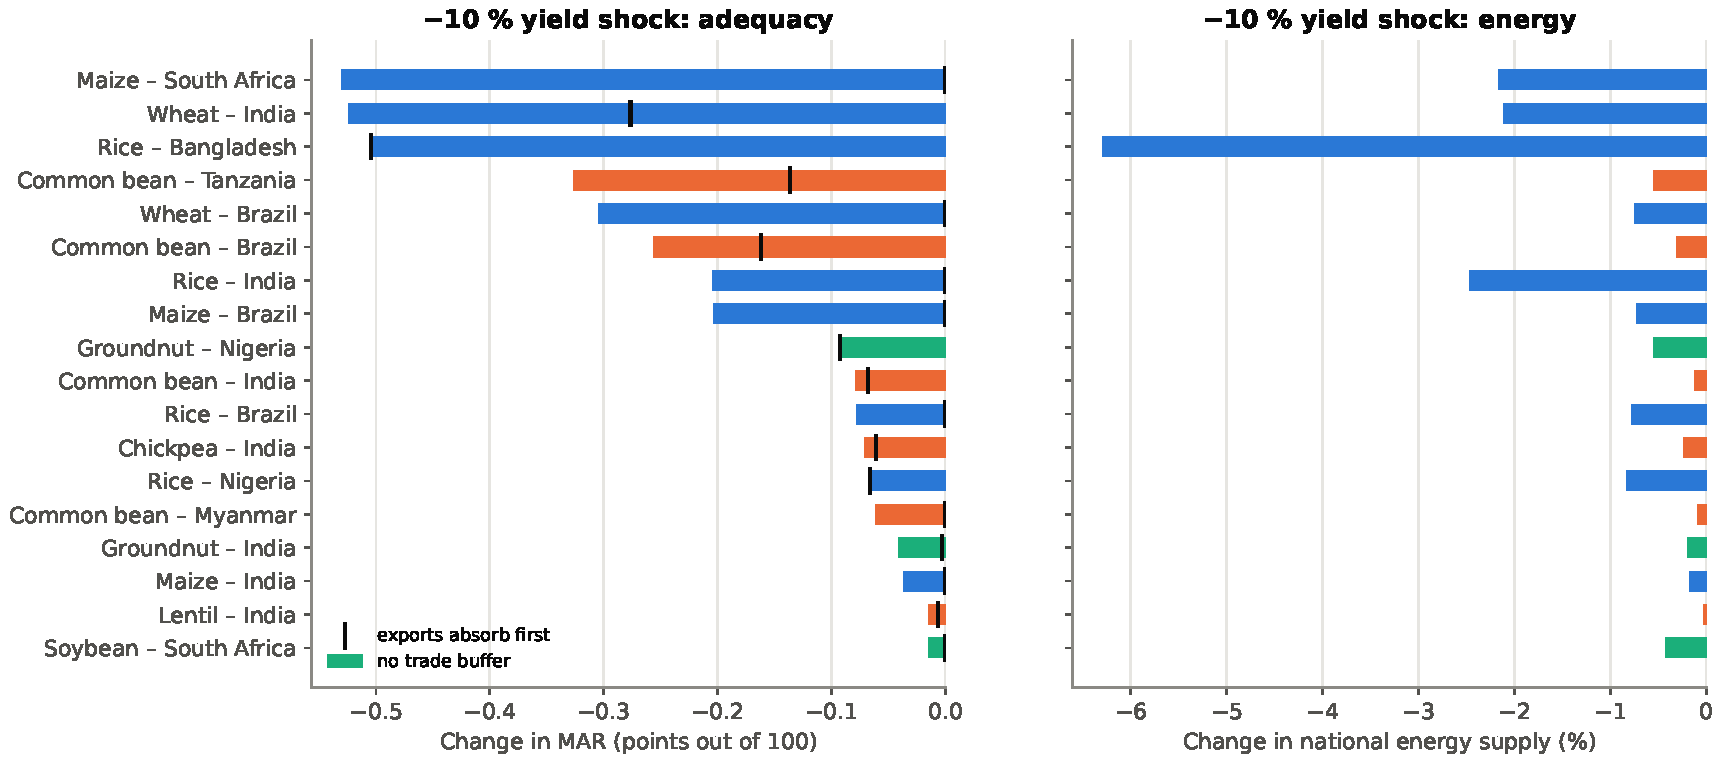
\includegraphics[width=0.9\linewidth]{G08_yield_shock.pdf}
\src{No market response; MAR caps each ratio at 1, so nutrient losses are shown too. Largest energy loss: \shockTopKcal\ (\shockTopKcalValue\%).}
\end{frame}

\begin{frame}{Future yield and nutrition: a conditional estimate}
\begin{columns}[T]
\column{0.55\textwidth}
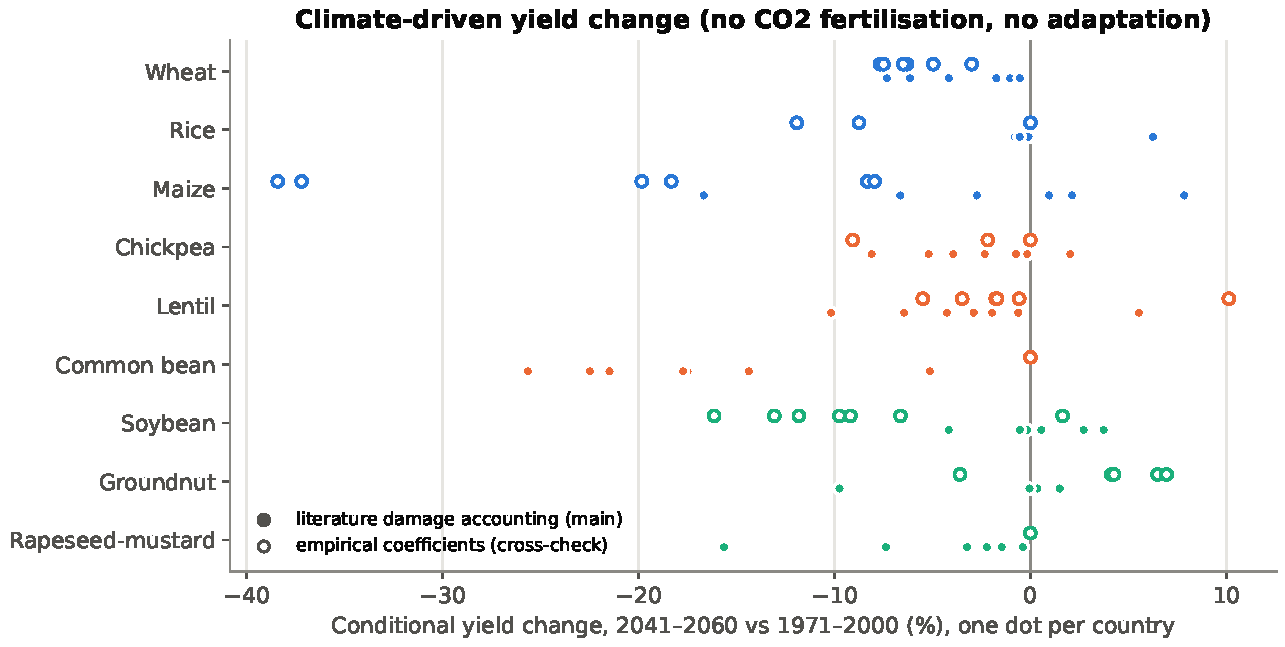
\includegraphics[width=\linewidth]{G09_future_yield.pdf}
\column{0.45\textwidth}\small
\begin{itemize}
\item Stress $\times$ literature response, paired before normalisation; only the change is used
\item Largest: \futYieldWorst\ (\futYieldWorstValue\% mean)
\item Empirical regressions do not confirm it pair by pair ($\rho$ = \corrLitEmp) $\Rightarrow$ screening estimate, not a forecast
\item No CO$_2$ fertilisation, adaptation or trade response
\end{itemize}
\end{columns}
\end{frame}

% India and Hyderabad slides (all numbers from numbers_india.tex)
\begin{frame}{India: what the nine-crop index says}
\begin{columns}[T]
\column{0.52\textwidth}\small
\textbf{Ranking for India:} \indOrder
\begin{itemize}
\item Wheat \indWheatFFour: \indWheatShIron\% of national iron, \indWheatShKcal\% of energy
\item Wheat today: mostly water; its \emph{future} rise is almost all heat
\item Chickpea \indChickpeaFFour: all water --- the highest rainfed deficit in the panel
\item 10\% wheat loss: energy \indWheatShockKcal\%, iron \indWheatShockIron\%, MAR \indWheatShockMar\ pts
\end{itemize}
\column{0.48\textwidth}\small
\textbf{A concentrated food supply}
\begin{itemize}
\item Effective food items supplying energy: India \divIndKcal, China \divChnKcal, USA \divUsaKcal, world \divWorldKcal
\item Cereals: \divIndCereal\% of energy
\item Wheat: largest iron source (\divIndIronTopShare\%)
\end{itemize}
\end{columns}
\src{FAO food balance sheets 2021--23 (Shannon diversity of supply, after Remans et al.\ 2014).}
\end{frame}

\begin{frame}{Hyderabad: a rice diet, unlike the national wheat story}
\begin{columns}[T]
\column{0.5\textwidth}\small
\textbf{Urban Telangana} (nearest official data to Hyderabad), kg per person per month
\begin{itemize}
\item Rice \hqTgUrbanKgRice\ vs wheat \hqTgUrbanKgWheat\ ($\times$\hqTgUrbanRiceToWheat; urban India $\times$\hqInUrbanRiceToWheat)
\item Cereals: \hqKcalCerealTgUrban\% of energy, \hqProtCerealTgUrban\% of protein
\item Protein-source diversity \hqProtEffTgUrban\ of 5 groups (urban India \hqProtEffInUrban)
\item Animal protein \hqProtAnimalTgUrban\% (India urban \hqProtAnimalInUrban\%)
\end{itemize}
\column{0.5\textwidth}\small
\textbf{Food groups, Telangana women: at least weekly}
\begin{itemize}
\item Pulses \hqWeeklyPulses\%, milk \hqWeeklyMilk\%, eggs \hqWeeklyEgg\%, meat \hqWeeklyMeat\%
\item Leafy vegetables \hqWeeklyLeafy\%, fruit \hqWeeklyFruit\%, fish \hqWeeklyFish\%
\end{itemize}
\textbf{Gaps:} fruit, leafy vegetables, fish
\end{columns}
\src{MoSPI HCES 2023--24 and NSS 594 (state, rural/urban); NFHS-5 Telangana state report (2019--21).}
\end{frame}

\begin{frame}{Nutrient diversity: where Hyderabad's iron comes from}
\begin{columns}[T]
\column{0.55\textwidth}\small
Share of iron from listed grains and pulses (HCES quantity $\times$ IFCT 2017):
\begin{itemize}
\item Rice \hqTgUrbanFeRice\% (urban India \hqInUrbanFeRice\%)
\item Wheat \hqTgUrbanFeWheat\% (urban India \hqInUrbanFeWheat\%)
\item Chickpea \hqTgUrbanFeChickpea\%, lentil \hqTgUrbanFeLentil\%, tur \hqTgUrbanFeTur\%, moong \hqTgUrbanFeMoong\%, groundnut \hqTgUrbanFeGroundnut\%
\end{itemize}
Rice: \SI{0.65}{mg} iron per \SI{100}{g}; chickpea and lentil dal 6.1--7.1.
\column{0.45\textwidth}\small
\textbf{Does the health data agree?} (NFHS-5, Hyderabad district)
\begin{itemize}
\item Anaemic: children \hydAnaemChild\%, non-pregnant women \hydAnaemNPW\%
\item Underweight women only \hydBmiLow\%; overweight/obese \hydOverweight\%
\end{itemize}
$\Rightarrow$ energy is adequate; \textbf{iron is the problem} --- the index's finding, locally.
\end{columns}
\src{Telangana, CNNS 2016--18: low ferritin \cnnsIronCFour\% (1--4 y), \cnnsIronAdol\% (adolescents); zinc deficiency \cnnsZincAdol\% (adolescents).}
\end{frame}

\begin{frame}{How would climate affect Hyderabad's diet?}
\begin{columns}[T]
\column{0.5\textwidth}\small
\textbf{Local climate} (grid cell; MRI-ESM2-0, SSP2-4.5)
\begin{itemize}
\item Mean $T_{\max}$ \hydTmaxBase\,$\to$\,\hydTmaxRecent\,\si{\celsius} (1971--2000 $\to$ 2001--24); rain \hydRainBase\,$\to$\,\hydRainRecent\,mm
\item 2041--60: April--May $T_{\max}$ $+$\hydAMFutChange\,\si{\celsius} (\hydAMFutLevel); rain \hydRainFutRatio\%
\end{itemize}
\textbf{Telangana crops}
\begin{itemize}
\item Rice: \tgAreaRice\% of cropland, \tgRiceRainfed\% rainfed $\Rightarrow$ almost no modelled stress
\item Paddy \tgPaddyAreaMha\,Mha (2023--24) vs \tgPaddySpamMha\,Mha in the 2010 map: $\times$\tgPaddyGrowth
\end{itemize}
\column{0.5\textwidth}\small
\textbf{Effect on iron from staples}
\begin{itemize}
\item Climate-driven yield change: rice \hqdYRice\%, chickpea \hqdYChickpea\%, wheat \hqdYWheat\% (national)
\item Iron from these foods: \hqIronChangeUrban\%
\item 10\% loss of rice: iron \hqIronTenRiceUrban\%; of wheat \hqIronTenWheatUrban\%
\end{itemize}
\begin{block}{Reading}Small next to the existing gap: Hyderabad's risk is structural; the climate route is irrigation, rainfed pulses and imported wheat.\end{block}
\end{columns}
\src{Conditional screening estimates; no CO$_2$ fertilisation, adaptation or market response.}
\end{frame}


\begin{frame}{Can we trust it?}
\begin{columns}[T]
\column{0.55\textwidth}
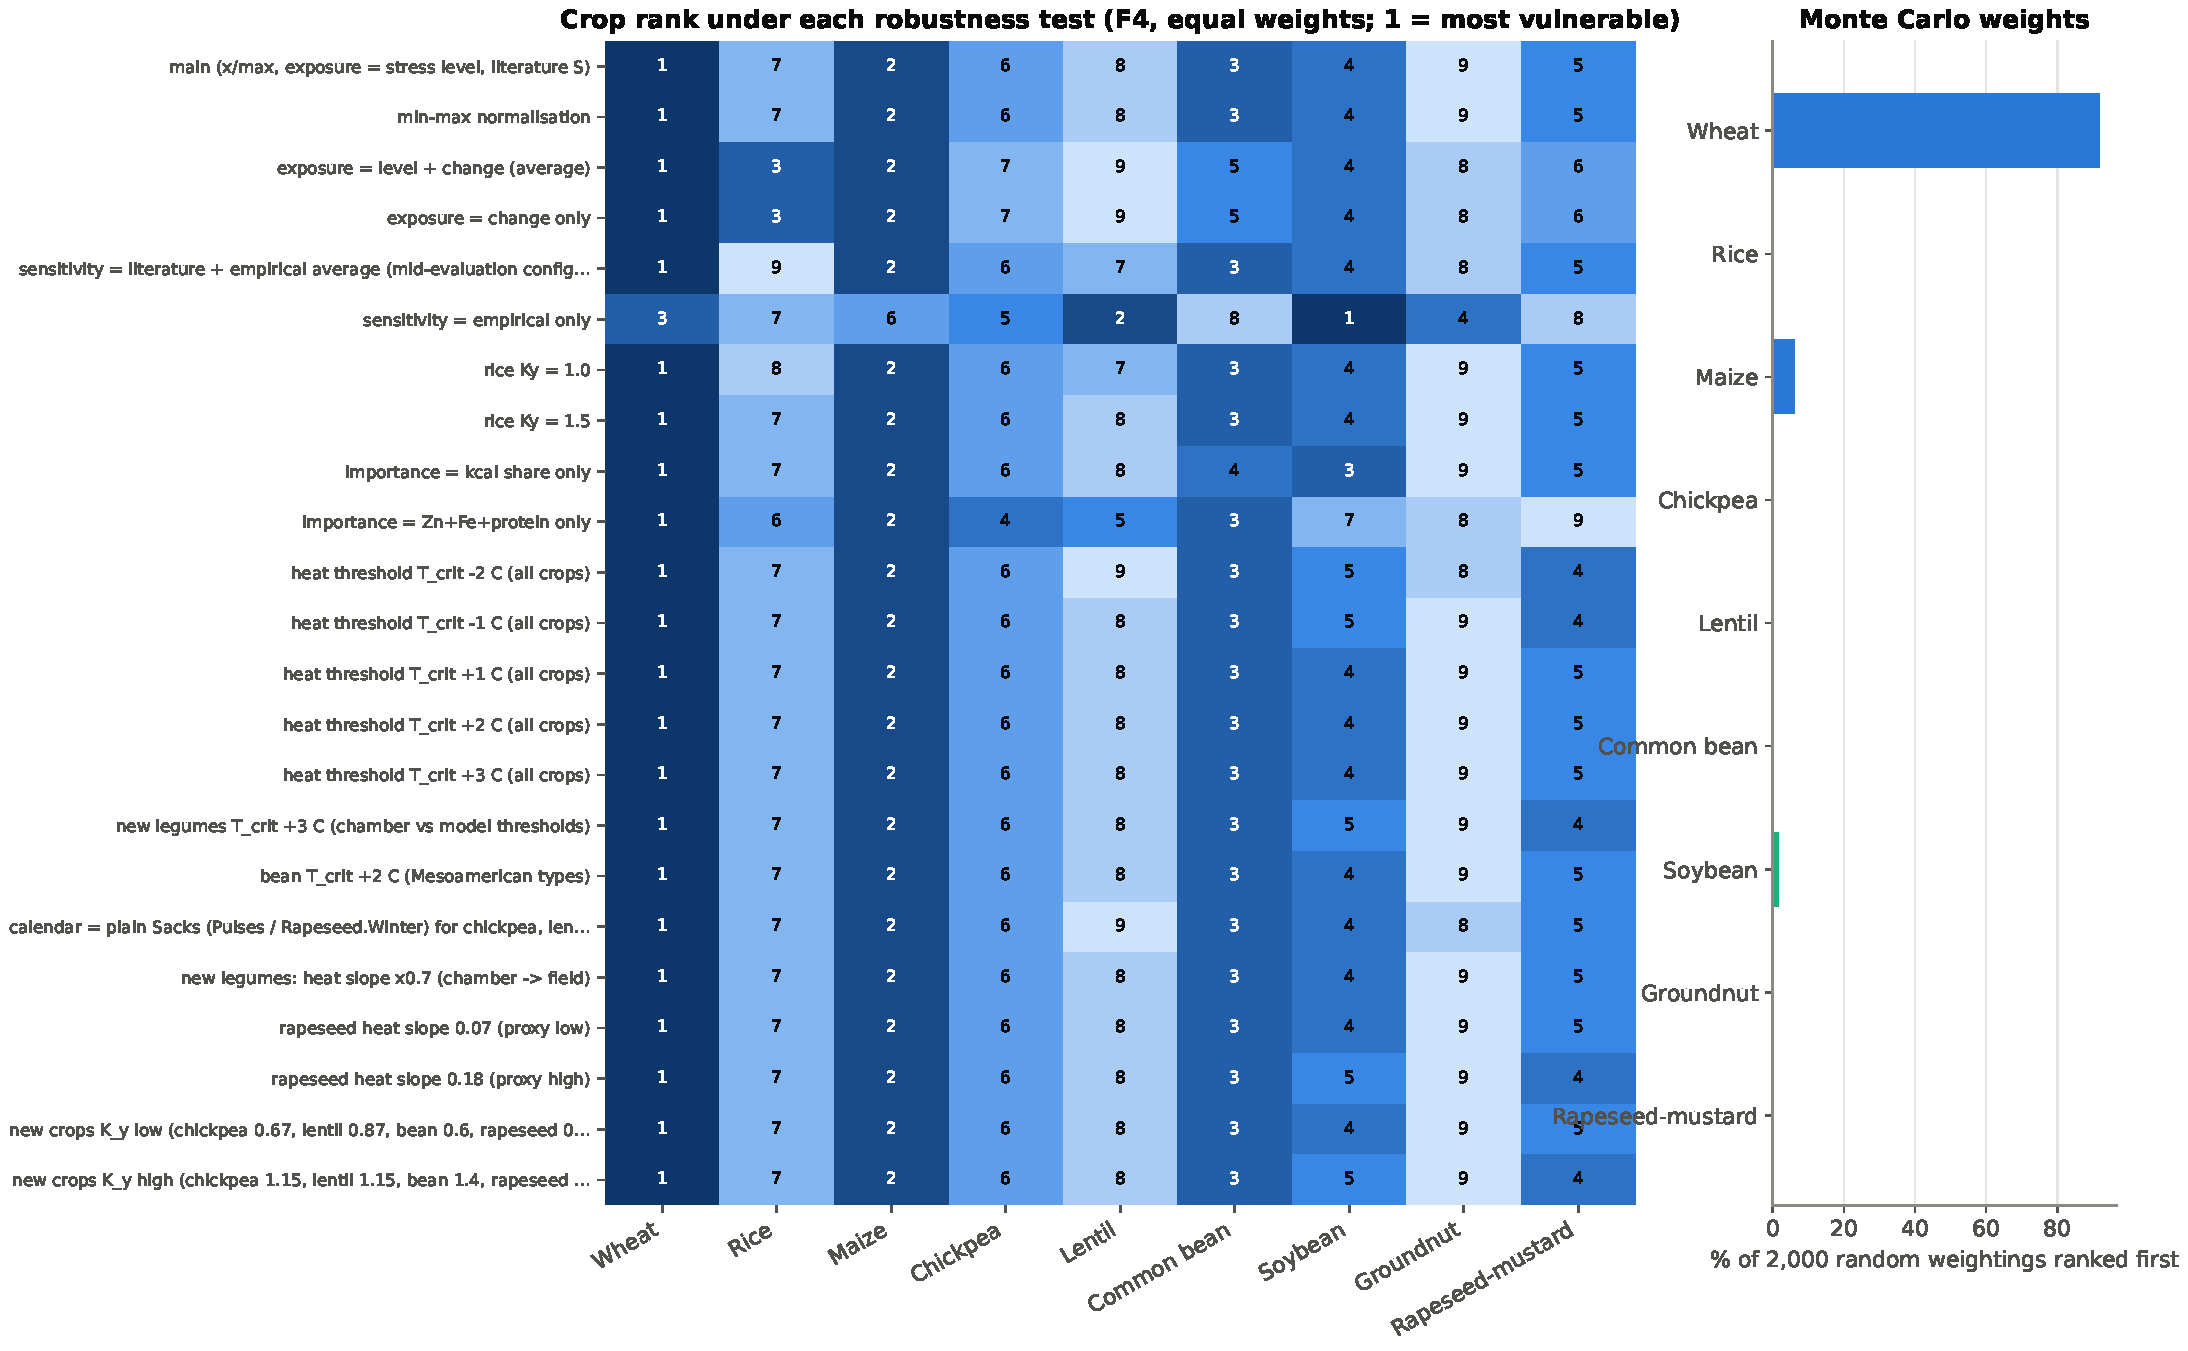
\includegraphics[width=\linewidth]{G10_robustness.pdf}
\column{0.45\textwidth}\small
\begin{itemize}
\item Wheat first in \robTopFfour\ of \robNFfour\ rankings (thresholds $\pm$3\,\si{\celsius}, calendars, proxies, weights)
\item First in \mcTopShare\% of 2,000 random weightings (share, not probability)
\item Positions 2--6 move with choices
\item Yield-shock test: $\rho$ = \shockRho\ ($p$ = \shockP, \shockNpairs\ pairs)
\item Literature: \litAgree\ of \litN\ comparisons agree, \litDiffer\ differ (Russia wheat mechanism; maize in Africa)
\end{itemize}
\end{columns}
\end{frame}

\begin{frame}{What the index indicates}
\begin{enumerate}
\item \textbf{Vulnerability is overlap}: wheat ranks first because it is stressed \emph{and} central to diets, not because it is most heat-sensitive
\item \textbf{Iron is the nutrient at stake}: climate risk falls on the nutrient already short
\item \textbf{Concentrated diets amplify}: India draws \divIndIronTopShare\% of its iron from wheat
\item \textbf{Irrigation is the hidden buffer} behind rice's low score
\item \textbf{Pulses rise fastest}: the protein and iron source of vegetarian diets
\end{enumerate}
\begin{block}{Points to}
heat-tolerant wheat and sowing dates in India; water management for rainfed maize and wheat; heat-tolerant beans; more diverse iron sources.
\end{block}
\end{frame}

\begin{frame}{Limitations}\small
\begin{itemize}
\item Monthly data: heat exposure is a lower bound; water ratio has no soil storage (overstates chickpea on residual moisture)
\item New-crop heat values are fits to chamber data; bean threshold from one Andean variety sets the heat reference
\item SPAM 2010 maps; gap-filled calendars; pigeon pea (tur) not among the nine crops
\item One climate model, one scenario
\item National supply $\neq$ individual intake; requirement choice changes the iron shortfall count
\item Future yield step: accounting, no CO$_2$ or adaptation; CO$_2$ nutrient effect shown only as an extra pathway
\end{itemize}
\end{frame}

\begin{frame}{Conclusion}
\begin{itemize}
\item \textbf{\topEq} is the crop whose climate stress most overlaps with its nutritional role --- robust across tests and to 2041--2060
\item Cereals most vulnerable; pulses rising fastest; iron is the nutrient at stake
\item India: wheat, chickpea and beans lead. Hyderabad: rice-based diet, so less exposed to the national wheat risk --- but rice is iron-poor and anaemia is already high; the climate route is irrigation, rainfed pulses and imported wheat
\item The index is a map of where adaptation and diet diversification would protect nutrition most
\end{itemize}
\end{frame}

\begin{frame}[allowframebreaks]{References}
\tiny\bibliography{refs}
\end{frame}

\appendix
\begin{frame}{Backup: worked example (wheat, India)}
\centering\scriptsize% worked example: wheat in India, from raw components to F4 (values from worked_example.csv via macros)
\begin{table}[t]
\centering\small
\caption{Worked example: wheat in India. The physical inputs are identical in both runs; only the
normalisation maxima differ. Values from \texttt{worked\_example.csv}; the hand calculation
$\tfrac12(E_TS_T+E_PS_P)\tilde I$ equals the pipeline value (checked by an assertion in the code).}\label{tab:worked}
\begin{tabular}{lrr}
\toprule
 & four-crop run & nine-crop run\\
\midrule
Heat level $L_{\text{heat}}$ (\si{\celsius} of $\Teff$ above \SI{25}{\celsius}) & \exFourLheatc & \exNineLheatc\\
\quad maximum over pairs & \exFourmaxLheat & \exNinemaxLheat\\
\quad $E_{\text{heat}}$ & \exFourEheat & \exNineEheat\\
Water level $L_{\text{water}}$ (rainfed share $\times$ deficit) & \exFourLwater & \exNineLwater\\
\quad maximum over pairs & \exFourmaxLwater & \exNinemaxLwater\\
\quad $E_{\text{water}}$ & \exFourEwater & \exNineEwater\\
Heat slope $s_T$ (/\si{\celsius}) and maximum over crops & \exFoursTpc\ / \exFourmaxsT & \exNinesTpc\ / \exNinemaxsT\\
\quad $S_T$ & \exFourSheat & \exNineSheat\\
$K_y$ and maximum over crops & \exFourKy\ / \exFourmaxKy & \exNineKy\ / \exNinemaxKy\\
\quad $S_P$ & \exFourSwater & \exNineSwater\\
Importance $I$ and maximum & \exFourI\ / \exFourmaxI & \exNineI\ / \exNinemaxI\\
\quad $\tilde I$ & \exFourInorm & \exNineInorm\\
\midrule
\Fd & \exFourFFourpipeline & \exNineFFourpipeline\\
\bottomrule
\end{tabular}
\end{table}

\end{frame}
\begin{frame}{Backup: presented method vs mid-evaluation numbers}
\centering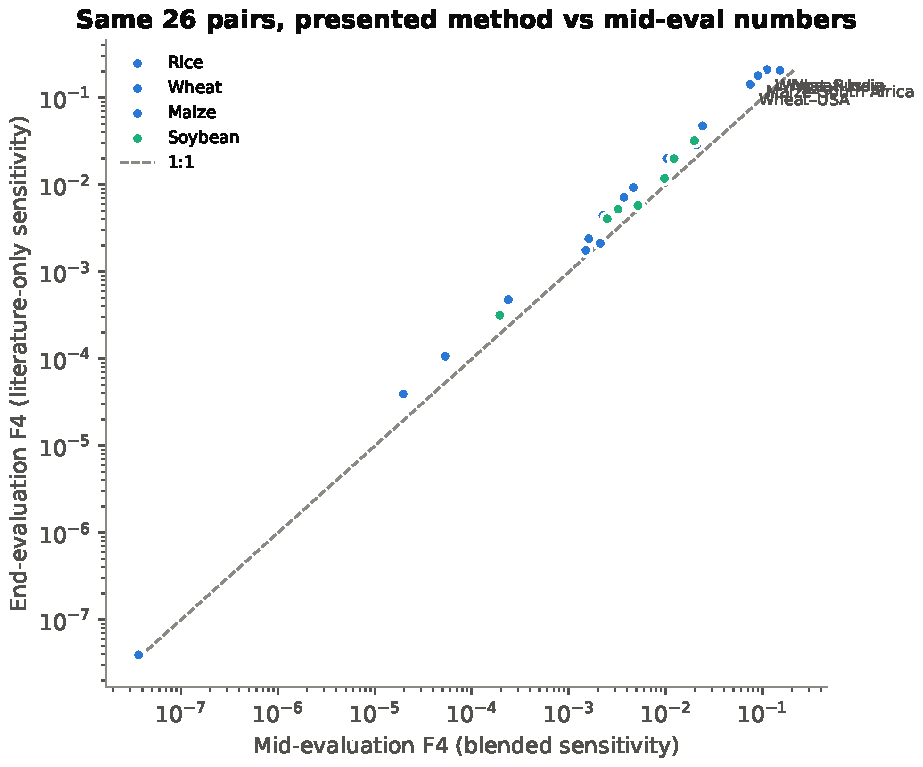
\includegraphics[height=0.8\textheight]{G11_mideval_vs_literature_only.pdf}
\src{Same 26 pairs; crop order unchanged (\orderFourEq); top pair now \litTopPair\ (\litTopValue) vs \litSecondPair\ (\litSecondValue).}
\end{frame}
\begin{frame}{Backup: largest future changes}
\centering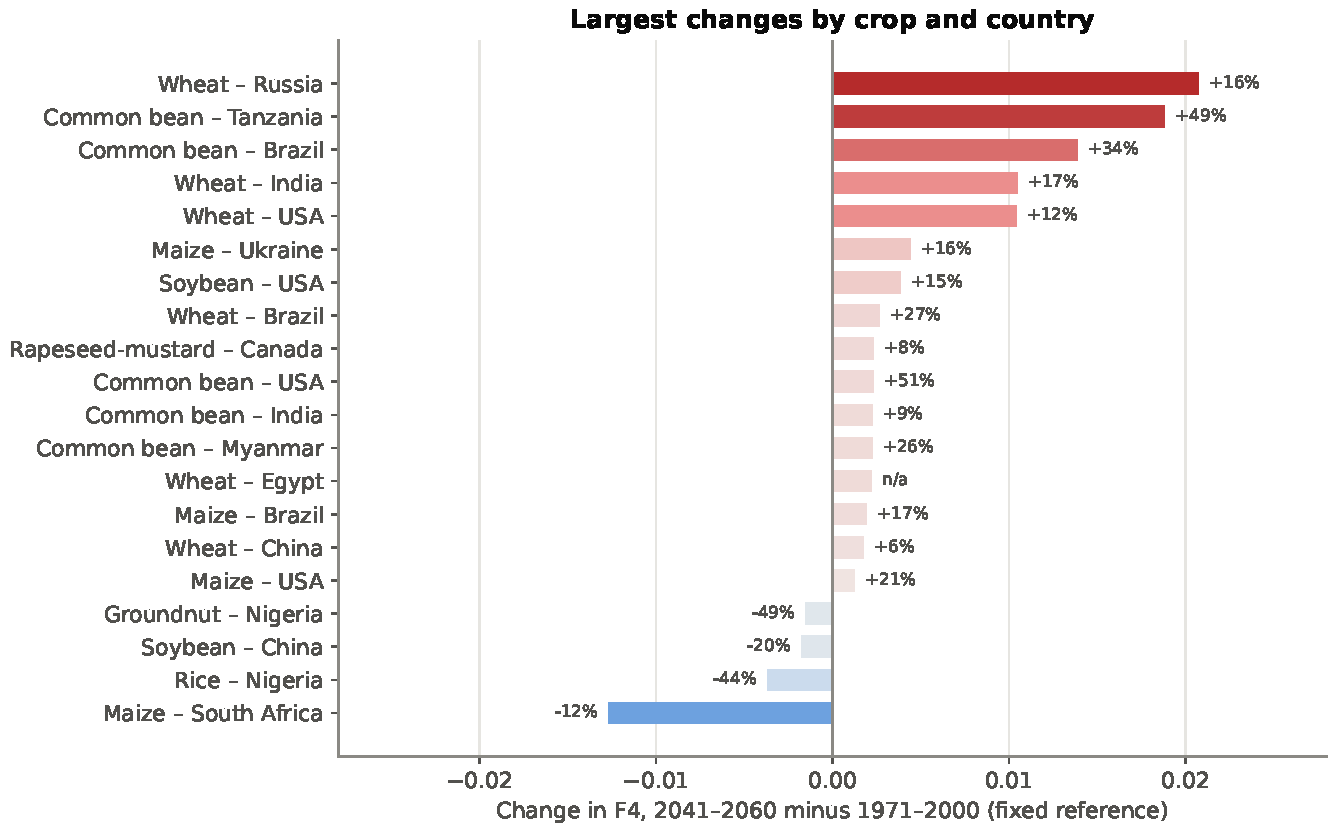
\includegraphics[height=0.8\textheight]{G05_future_pairs.pdf}
\end{frame}
\end{document}
